\documentclass{article}
\usepackage{amsmath}
\usepackage{hyperref,graphicx,natbib}
\hypersetup{
  colorlinks   = true,    % Colours links instead of ugly boxes
  urlcolor     = blue,    % Colour for external hyperlinks
  linkcolor    = blue,    % Colour of internal links
  citecolor    = black      % Colour of citations
}

\usepackage{etoolbox}

\makeatletter

\pretocmd{\NAT@citex}{%
  \let\NAT@hyper@\NAT@hyper@citex
  \def\NAT@postnote{#2}%
  \setcounter{NAT@total@cites}{0}%
  \setcounter{NAT@count@cites}{0}%
  \forcsvlist{\stepcounter{NAT@total@cites}\@gobble}{#3}}{}{}
\newcounter{NAT@total@cites}
\newcounter{NAT@count@cites}
\def\NAT@postnote{}

% include postnote and \citet closing bracket in hyperlink
\def\NAT@hyper@citex#1{%
  \stepcounter{NAT@count@cites}%
  \hyper@natlinkstart{\@citeb\@extra@b@citeb}#1%
  \ifnumequal{\value{NAT@count@cites}}{\value{NAT@total@cites}}
    {\ifNAT@swa\else\if*\NAT@postnote*\else%
     \NAT@cmt\NAT@postnote\global\def\NAT@postnote{}\fi\fi}{}%
  \ifNAT@swa\else\if\relax\NAT@date\relax
  \else\NAT@@close\global\let\NAT@nm\@empty\fi\fi% avoid compact citations
  \hyper@natlinkend}
\renewcommand\hyper@natlinkbreak[2]{#1}

% avoid extraneous postnotes, closing brackets
\patchcmd{\NAT@citex}
  {\ifNAT@swa\else\if*#2*\else\NAT@cmt#2\fi
   \if\relax\NAT@date\relax\else\NAT@@close\fi\fi}{}{}{}
\patchcmd{\NAT@citex}
  {\if\relax\NAT@date\relax\NAT@def@citea\else\NAT@def@citea@close\fi}
  {\if\relax\NAT@date\relax\NAT@def@citea\else\NAT@def@citea@space\fi}{}{}

\makeatother

\DeclareMathOperator\erf{erf}
\title{A Rough Guide to CladeAge\\
{\small Bayesian  estimation of clade ages based on probabilities of fossil sampling}}
\author{Michael Matschiner \\
\href{mailto:michaelmatschiner@mac.com}{michaelmatschiner@mac.com}\vspace{1.5 mm}\\
Remco Bouckaert\\ 
\href{mailto:remco@cs.auckland.ac.nz}{remco@cs.auckland.ac.nz}}

\begin{document}
\maketitle
\begin{center}
\includegraphics[width=0.3\textwidth]{cladeage_256x256px.png}\end{center}
\tableofcontents

\section{Introduction}

\subsection{Summary}
CladeAge is an add-on package for the Bayesian software BEAST 2 \citep{Bouckaert:2014ii} which allows time calibration of phylogenetic trees based on probability densities for clade ages, calculated from a model of constant diversification and fossil sampling.

\subsection{Background}
In Bayesian node dating, phylogenies are commonly time calibrated through the specification of calibration densities on nodes representing clades with known fossil occurrences. Unfortunately, the optimal shape of these calibration densities is usually unknown and they are therefore often chosen arbitrarily, which directly impacts the reliability of the resulting age estimates. CladeAge overcomes this limitation by calculating optimal calibration densities for clades with fossil records, based on estimates for diversification rates and the sampling rate for fossils. This rate characterizes the frequency, at which fossils are preserved along branches of a phylogeny, and only fossils that are ultimately sampled (and published) by researchers are used for this measure. 

\subsection{Reference}
A manuscript describing the CladeAge model is accepted (pending revision) for publication in Systematic Biology, and a preprint can be found on BioRxiv:\vspace{1.5 mm} \\
Matschiner M, Musilov\'{a} Z, Barth JMI, Starostov\'{a} Z, Salzburger W, Steel M, Bouckaert R (2016) Bayesian node dating based on probabilities of fossil sampling supports trans-Atlantic dispersal of cichlid fishes, BioRxiv preprint, doi: \href{https://doi.org/10.1101/038455}{https://doi.org/10.1101/038455}.

\subsection{Contact}
If this guide still leaves questions you can contact the authors,
or consult the BEAST user list on \href{http://groups.google.com/group/beast-users}{http://groups.google.com/group/beast-users}.

\section{CladeAge calibration densities}

CladeAge calculates probability densities for the age of origin of a clade, given the age of its oldes fossil, based on an assumed model of constant diversification and fossil sampling. Under the further assumption that the age of origin of a clade is equivalent to the divergence time between this clade and its sister lineage, these probabilities can be used as calibration densities for Bayesian divergence-time estimation. The performance of CladeAge calibration densities for divergence-time estimation has been tested extensively with simulated and empirical datasets \citep{Matschiner:2016ga}. The CladeAge model includes four required parameters (the first occurrence age, net diversification rate, turnover rate, and sampling rate) and one optional parameter (the sampling gap), which are described below. Note that ranges can be specified for all parameters to account for uncertainties in their estimates.

\subsection{CladeAge model parameters: the first occurrence age}\label{first_occurrence_age}

The first occurrence age of a clade is the age of the oldest fossil that can be reliably assigned to this clade. For example, the oldest currently known fossil taxon that can be assigned to cetaceans (whales) is $\dagger$\textit{Himalayacetus subathuensis} from the Indian Suba\-thu Formation \citep{Benton:2015wj}. Within this formation, the fossil was found in a layer characterized by the occurrence of the foraminifer \textit{Nummulites atacicus} \citep{Bajpai:1998wm}, which allows correlation with the Shallow Benthic Zone (SBZ) 8 \citep{Vandenberghe:2012ih}. The ages of the boundaries of SBZ8 are not directly defined \citep{Vandenberghe:2012ih}, but SBZ 8 is usually considered to correspond to nannoplankton zones NP10-11, and these are known to span 56.0-53.5 Ma \citep{Vandenberghe:2012ih}. Thus, the first occurrence age of cetaceans is 56.0-53.5 Ma.

As becomes obvious from this example, the identification of the first occurrence age from the systematic, paleontological, and geological literature is not always straightforward. However, some excellent starting points for this investigation are \citet{Benton:2015wj}, the Fossil Calibration Database (\href{http://fossilcalibrations.org}{http://fossilcalibrations.org}), and the Paleobiology Database (\href{https://paleobiodb.org}{https://paleo-\linebreak biodb.org}). For conversions to absolute ages, the book \emph{The Geologic Time Scale 2012} \citep{Gradstein:2012ur} is highly recommended, but should be complemented with the latest version of the International Chronostratigraphic Chart, published by the International Commission on Stratigraphy (\href{http://stratigraphy.org/index.php/ics-chart-timescale}{http://stratigraphy.org/index .php/ics-chart-timescale}).

Similar to $\dagger$\textit{Himalayacetus subathuensis}, nearly all fossil ages are associated with uncertainties that often can be considered uniform within lower and upper boundaries. By specifying these boundaries as input for CladeAge, the uncertainty in first occurrence ages can (and should) be accounted for.

\subsection{CladeAge model parameters: the diversification rates}\label{diversification_rates}

To estimate the total phylogenetic history of a clade prior to the preservation of its oldest fossil record, CladeAge implements a birth-death model of constant diversification. Thus, the model includes both a speciation rate $\lambda$ and an extinction rate $\mu$. However, as diversification rates are more easily estimated, and more commonly reported in the literature as net diversification rate $\lambda - \mu$ and turnover rate $\mu / \lambda$, CladeAge is written to accept as input net diversification rate and turnover rate, rather than speciation rate and extinction rate (internally, it then uses the specified net diversification rate and turnover rate to calculate speciation and extinction rates). If diversification rates for the clade of interest have not previously been reported in the literature, these can be estimated either from the fossil record alone or from separate phylogenies, using software such as BAMM \citep{Rabosky:2014ba}, RPANDA \citep{Morlon:2015jm}, MEDUSA \citep{Alfaro:2009vc}, TRiPS \citep{Starrfelt:2016en}, PyRate \citep{Silvestro:2014ga}, or paleotree \citep{Bapst:2012hg}.

\subsection{CladeAge model parameters: the sampling rate}\label{sampling_rate}

Probability densities calculated with CladeAge are based on estimates of the sampling rate $\psi$ of fossils, assuming that sampling is a constant Poisson process. The concept of a sampling rate of fossils is commonly used in the paleontological literature, and is considered to include all processes that lead to the identification and scientific description of a fossil. Thus, the sampling rate encompasses deposition of an organism in the sediment, fossilisation, survival of geological processes, outcropping of the rock formation including the fossil, discovery, correct taxonomic identification, and publication of the fossil find.

Estimates of sampling rates can be obtained by a variety of methods, including the freqRat method of \citet{Foote:1996tf}, the survivorship analysis of \citet{Foote:2001js}, and the analysis of waiting times between sampling events, introduced by \citep{Solow:1997tba}. All these methods have in common that a very large number of fossils, and ideally full occurrence data, i.e., information for each known fossil of a given group, is needed for reliable sampling rate estimates. Thus, for most studies aiming to time-calibrate phylogenies, the estimation of sampling rates for the investigated group is beyond the scope of the analysis. Fortunately however, sampling rates have already been estimated and published for many groups and can readily be used in CladeAge. For example, \citet{Foote:1999ts} estimated the sampling rate of Late Cretaceous mammals as 0.03-0.06, \citet{Alba:2001va} found the sampling rate of Iberian mammals of the Neogene to be around 0.8, and \citet{Foote:1996tf} determined the sampling rate of European Jurassic bivalves to be around 0.41 (all values given are per lineage and per million years).

Previously, sampling rates have often been published on genus level instead of species level, and not per million years, but for shorter or longer time bins \citep{Foote:1996tf,Foote:1999vr,Friedman:2011es}. In order to use these estimates in CladeAge, they must be transformed into species-level estimates per million years (assuming that fossil ages are also specified in million years in BEAST). One way to transform genus level estimates into species level estimates is to calculate the average number of extant species per genus in the investigated group, assuming that this ratio also holds for fossil members of the same group. If rates have been given for time bins other than a million years, the rate conversion can be performed e.g.\ with the function \emph{Prob2sRate} of the R package paleotree \citep{Bapst:2012hg}. A compilation of published species-level sampling rate estimates for diverse groups of organisms can be found in Supplementary Table S1 of \citet{Matschiner:2016ga}.

\subsection{CladeAge model parameters: the sampling gap}\label{sampling_gap}

As an optional parameter, a sampling gap can be specified. The sampling gap represents the time period at the very beginning of a clade's history, for which one can assume that the clade's preservation potential was negligible, effectively setting the sampling rate $\psi$ to zero for this period. There are several reasons why one might assume the existence of a sampling gap: For example, the populations sizes of a clade might have been very small shortly after its origination, which could have reduced its potential to become preserved in the fossil record. Similarly, if the population has been geographically limited to a small region, which is more likely at the beginning of a clade's history, this would also lower its preservation potential. One might also assume that clades require time to evolve morphological features that allow fossils to be assigned to these clades. As the sampling rate $\psi$ includes all processes from the fossilisation of an organism to its discovery and correct taxonomic assignment, $\psi$ would also be zero for the time before the emergence of recognisable morphological features of a clade.

Whether or not a sampling gap should be used in CladeAge analyses is debatable, as one might argue that over time periods of millions of years, as are usually considered in divergence-time estimation, the times required to reach substantial population sizes and geographic distributions, or to evolve recognisable morphological features, are negligible. In fact, the latter may even go simultaneously with clade origination according to the theories of punctuated equilibrium and key innovations \citep{Pennell:2013ij,Rabosky:2013by}. Note that a sampling gap was not used in combination with simulated datasets in \citet{Matschiner:2016ga} and the performance of CladeAge with specified sampling gaps has not yet been tested.

\subsection{Units}

Note that the units used for calibrations should match those used for other parts of the model, so if you specify the parameters of the CladeAge model in millions of years, the clock prior should be in million of years as well. Obviously, the tree will then be interpreted in millions of years as well.

\section{Applying CladeAge calibration densities}

\subsection{Which fossils to use}

CladeAge calibration densities describe the probabilities for the age of a clade, given the age of its first occurrence. Thus, \textbf{only the oldest fossil of a clade should be used} for the specification of CladeAge calibration densities, and younger fossils of the same clade should be ignored. Obviously, there should be morphological evidence that the putatively oldest fossil record of a clade is in fact a member of that clade. Based on morphology, the general assignment of fossils to clades (regardless of the fossil's position within the clade) is usually more robust than determining whether or not the fossil is a member of the crown or stem group of that clade. Therefore, CladeAge calibration densities are designed to be applied to the origin of a clade regardless of whether its oldest fossil is part of the stem group or the crown group of the clade.

\subsection{Which clades to use}

In practice, it may not always be clear which clades in a phylogeny should be used for time calibration: If a fossil represents the earliest record of not only one clade, but of multiple nested clades, CladeAge calibration densities could be used to constrain the age of origin of all these clades, only of the most inclusive of these clades, or only of the least inclusive clade. Furthermore, if two sister clades both possess a fossil record, these fossils could be used to constrain the ages of both of the two clades. However, as the ages of the two clades are necessarily linked by their simultaneous divergence, two time constraints would effectively be placed on one and the same node. Instead, it may seem more intuitive to use only the older of the two fossils for time calibration and disregard the younger fossil. Thus, a number of schemes could be chosen to select clades for calibration (illustrated in Fig.\ 2 of \citealt{Matschiner:2016ga}). The performance of these calibration schemes was tested in \citet{Matschiner:2016ga} with a wide range of simulated datasets. Based on the results of these analyses, we recommend a calibration scheme according to which fossils are used to strictly constrain all clades, for which these fossils represent the oldest known record (see Fig.\ 1 on the next page). This means that some \textbf{fossils may be used to constrain the ages of more than one of several nested clades}, particularly if groups with poor fossil records are investigated. It also means that constraints on clade ages should be applied irrespective of the fossil record of the sister group of the clade. Thus, even if the sister group has older fossil records, the oldest fossil of a clade should still be used as a constraint. A positive aspect of this is that sister groups do not need to be known before the analysis, unlike in traditional node-dating approaches.

Thus, \textbf{CladeAge calibration densities should be applied to all clades that have a fossil record, and bias would be introduced if only clades with particularly old (or young) fossils would be used}. There are two exceptions to this rule:

\begin{enumerate}
\item For clades that are recovered in phylogenies, but are not supported by morphological synapomorphies, the sampling rate is effectively reduced to zero, as it would be impossible to assign fossils directly to these clades based on morphology. Indirectly, these clades might still have a fossil record as it may be possible to assign fossils to subclades that are characterized by morphological synapomorphies. Nevertheless, these clades should not be constrained with fossils assigned to subclades \citep[see][for a more detailed discussion of this case]{Matschiner:2016ga}.
\item While it is not necessary to know the sister group of calibrated clades, the sister group should still be included in the dataset. If the true sister group of a calibrated clade was instead missing from a phylogeny, the origin of the branch leading to the calibrated clade would be older than the clade itself, which would violate assumptions made when using CladeAge probability densities as calibration densities in BEAST 2. Thus, in this case, the age of the clade should not be constrained. To ensure that a clade's sister group is included in the phylogeny even if the identity of the sister group is not known, one could simply include representatives of all possible sister groups in the dataset. Missing sister groups can be avoided completely if so-called \emph{diversity trees} \citep{Alfaro:2009vc} are used for the analysis, where each extant species of a given group can be assigned to one of the tips of the phylogeny.
\end{enumerate}

\noindent
\begin{figure}[h!]
   \centering
   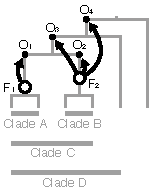
\includegraphics[width=35 mm]{fig1}
\end{figure}\\
\textbf{Figure 1:} Calibration scheme to be used with CladeAge calibration densities.\\
When using CladeAge calibration densities, fossils should be used as constraints for the age of origin of all clades, for which the fossil represents the oldest known record. Here, fossils F$_1$ and F$_2$, represented by white circles, are the oldest fossils of clades A and B, respectively, and no fossils are known outside of these two clades. As F$_2$ is older than F$_1$ it also represents the oldest record of clades C and D. Thus, F$_1$ should be used to constrain the age of clade A (marked with a black dot and the label O$_1$), and F$_2$ should be used to constrain the age of origin of clades B, C, and D (marked with O$_2$, O$_3$, and O$_4$). Note that since clades A and B are sister lineages, O$_1$ and O$_2$ are identical in age.
\newpage


\section{Installing CladeAge}

\subsection{Using BEAUti}\label{using_beauti}

Like other add-on packages for BEAST 2, CladeAge can be installed through the package manager that's built into BEAUti, a utility tool that comes with the BEAST 2 download (see \href{http://beast2.org}{http://beast2.org} for details). To install CladeAge, open BEAUti, and select \emph{Manage Packages} from the File menu:

\begin{center}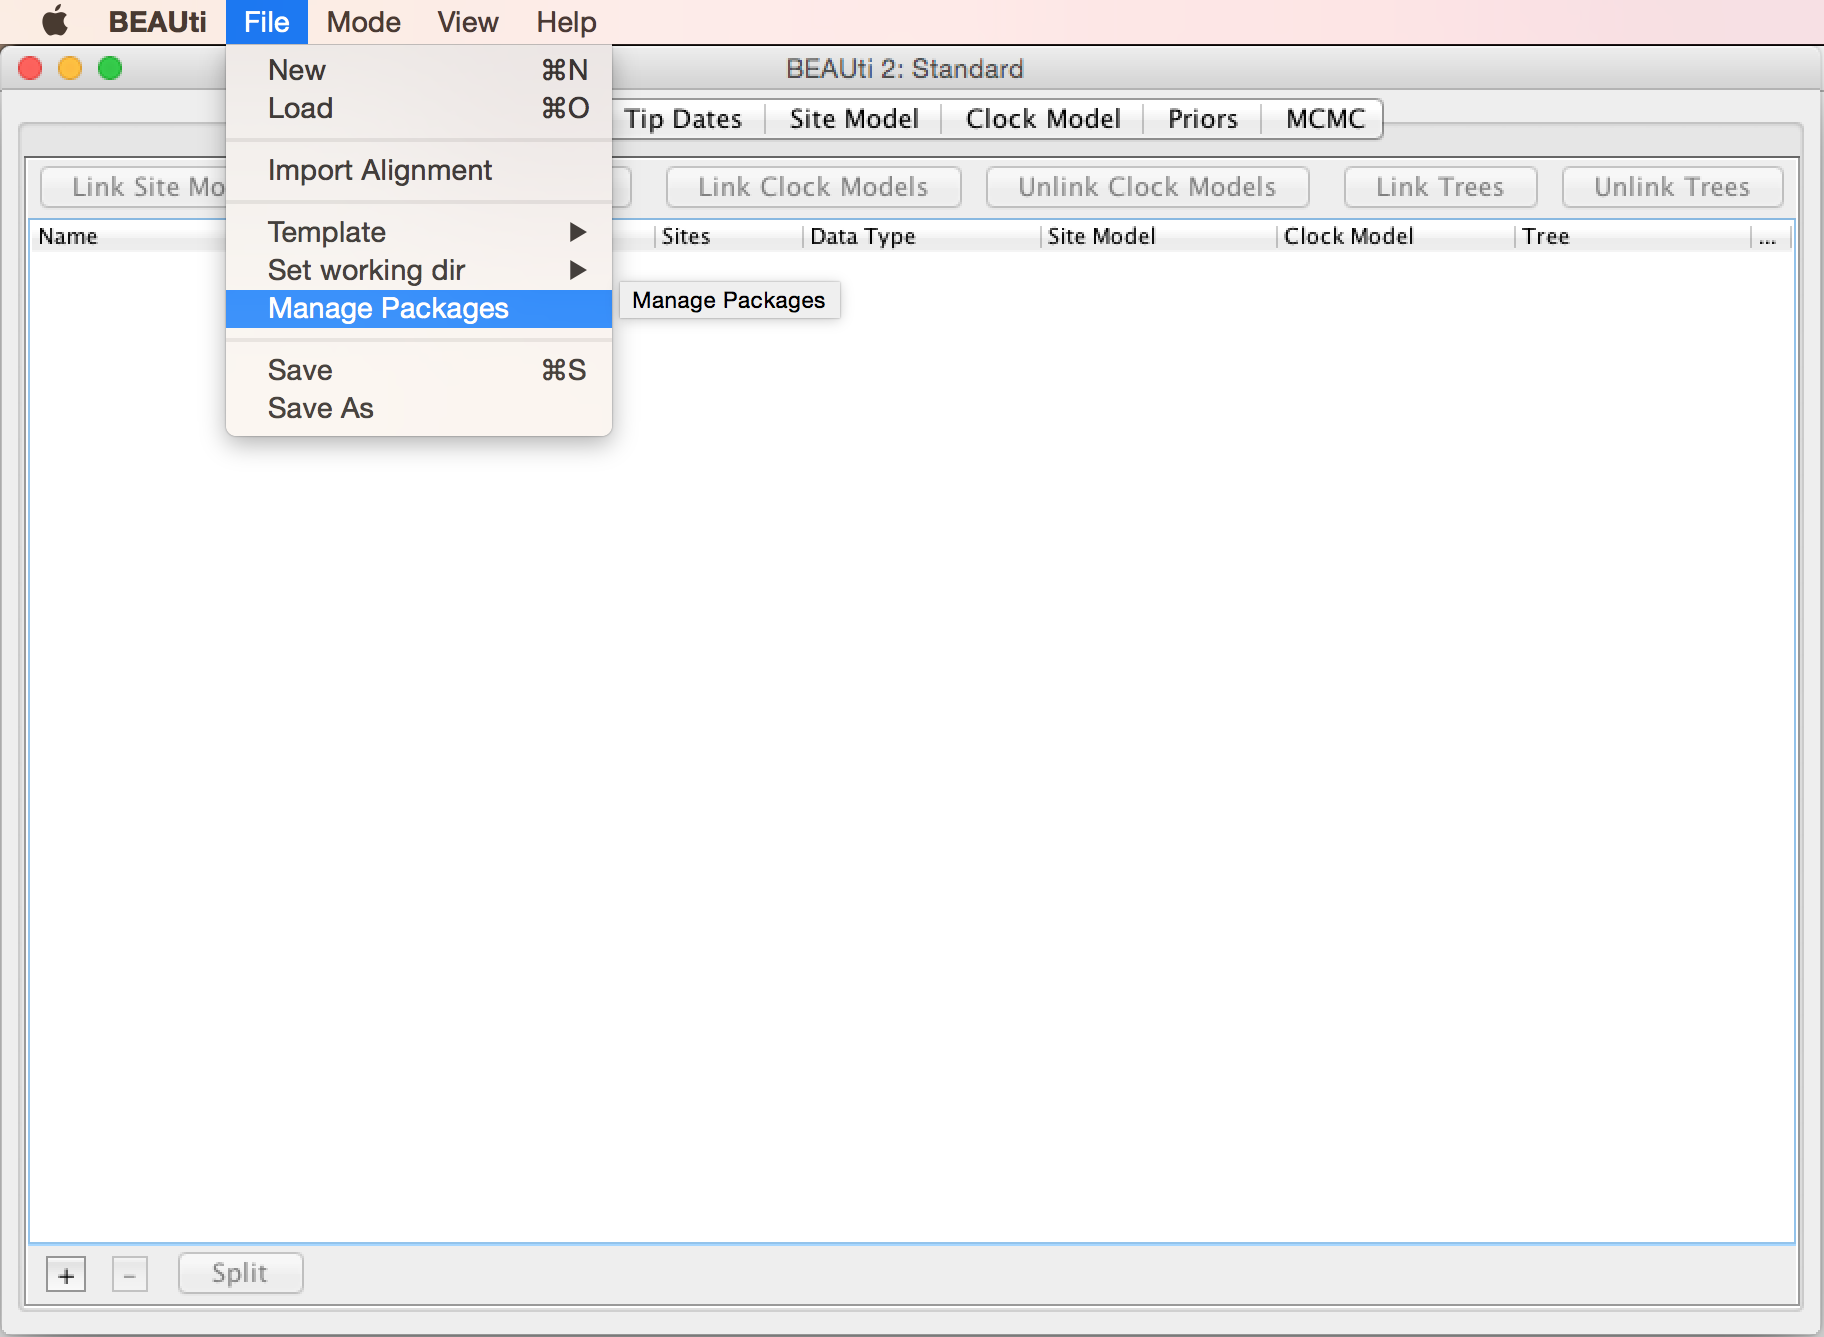
\includegraphics[width=\textwidth]{fig2.png}\end{center}

\noindent
Then select the \emph{CA} package from the list and click the Install/Upgrade button:

\begin{center}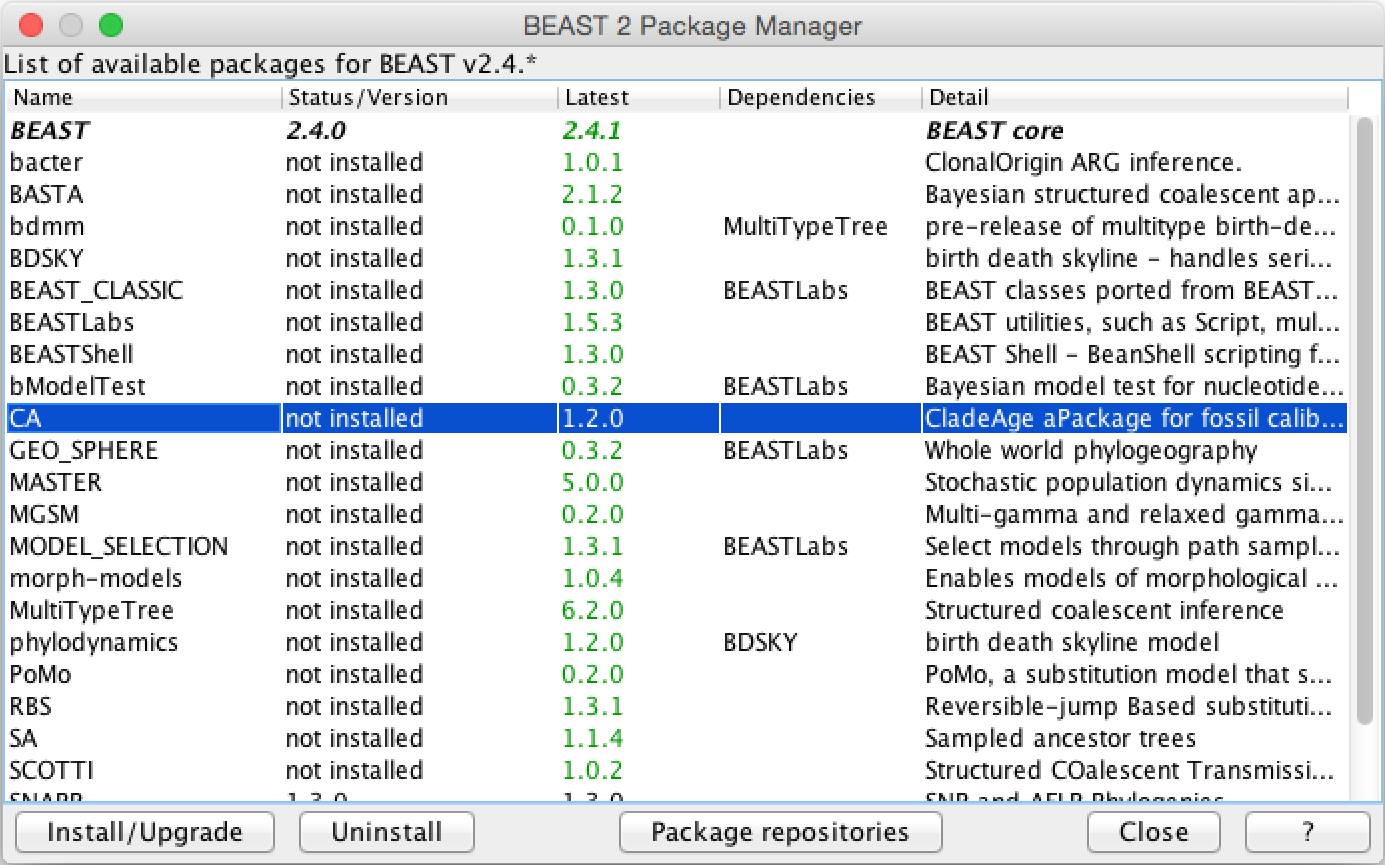
\includegraphics[width=0.76\textwidth]{fig3.png}\end{center}

\noindent
Restart BEAUti, and a new panel for \emph{Clade Ages} should have appeared, as you can see from the buttons in the top row of the BEAUti window:

\begin{center}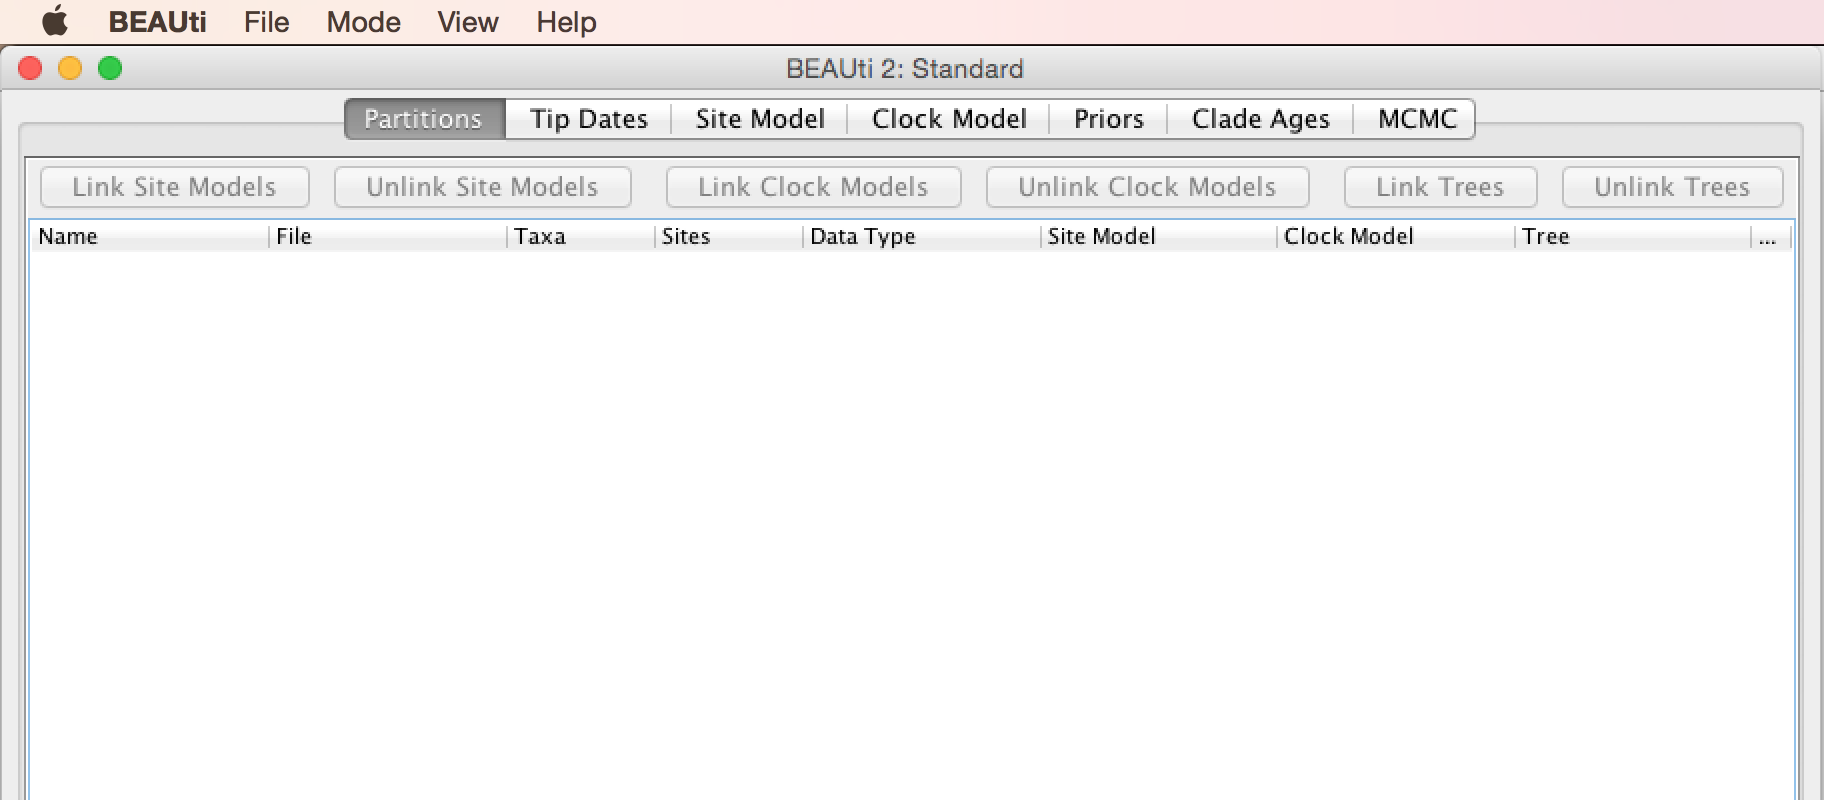
\includegraphics[width=\textwidth]{fig4.png}\end{center}

\noindent
The \emph{Clade Ages} panel is where you can specify rate estimates for speciation, extinction, and fossil sampling, and CladeAge calibration densities will be automatically calculated based on these parameters (see below).

\subsection{Using the command line}

Alternatively, you can use the command-line utility \emph{addonmanager} to install CladeAge (or other packages for BEAST 2), which is useful for cluster computers without GUI access. To see the available options, type

\footnotesize
\begin{verbatim}
PATH_TO_BEAST/bin/addonmanager
\end{verbatim}
\normalsize

\noindent
in a console window (make sure to replace \emph{PATH\_TO\_BEAST} with the actual path to the BEAST 2 directory). You should see the following output:

\footnotesize
\begin{verbatim}
  Usage: addonmanager [-list] [-add <NAME>] [-del <NAME>] [-useAppDir]
    [-dir <DIR>] [-help] 
  -list List available add-ons
  -add Install the <NAME> add-on 
  -del Uninstall the <NAME> add-on 
  -useAppDir Use application (system wide) installation directory. Note this
    requires writing rights to the application directory. If not specified,
    the user's BEAST directory will be used.
  -dir Install/uninstall add-on in directory <DIR>. This overrides the useAppDir
    option
  -help Show help
\end{verbatim}
\normalsize

\noindent
To install the CladeAge package with \emph{addonmanager}, use

\footnotesize
\begin{verbatim}
PATH_TO_BEAST/bin/addonmanager -add CA
\end{verbatim}
\normalsize

\subsection{Manual installation}

If for some reason installation with BEAUti or \emph{addonmanager} is not possible, you can also install the CladeAge package manually. To do so, download the latest version of the compressed CladeAge package (named \emph{CA.addon.vX.X.X.zip}, where \emph{X.X.X} is a version number) from \href{https://github.com/CompEvol/CBAN/releases}{https://github.com/CompEvol/ \linebreak CBAN/releases}. Uncompress the package, and place the directory \emph{CA} in one of the following locations, depending on your operating system (make sure to replace \emph{USERNAME} with your user name, and \emph{X} with the version number of BEAST 2).\\

\noindent
Windows: \footnotesize\verb!Users\USERNAME\BEAST\2.X!\normalsize

\noindent
Mac: \footnotesize\verb!/Users/USERNAME/Library/Application Support/BEAST/2.X!\normalsize

\noindent
Linux: \footnotesize\verb!/home/USERNAME/.beast/2.X!\normalsize


\section{Specifying CladeAge calibration densities}

\subsection{Using BEAUti}

To specify a new CladeAge calibration density in BEAUti, open the \emph{Clade Ages} tab (after you imported a sequence alignment with \emph{Import Alignment} in the \emph{File} menu).

\begin{center}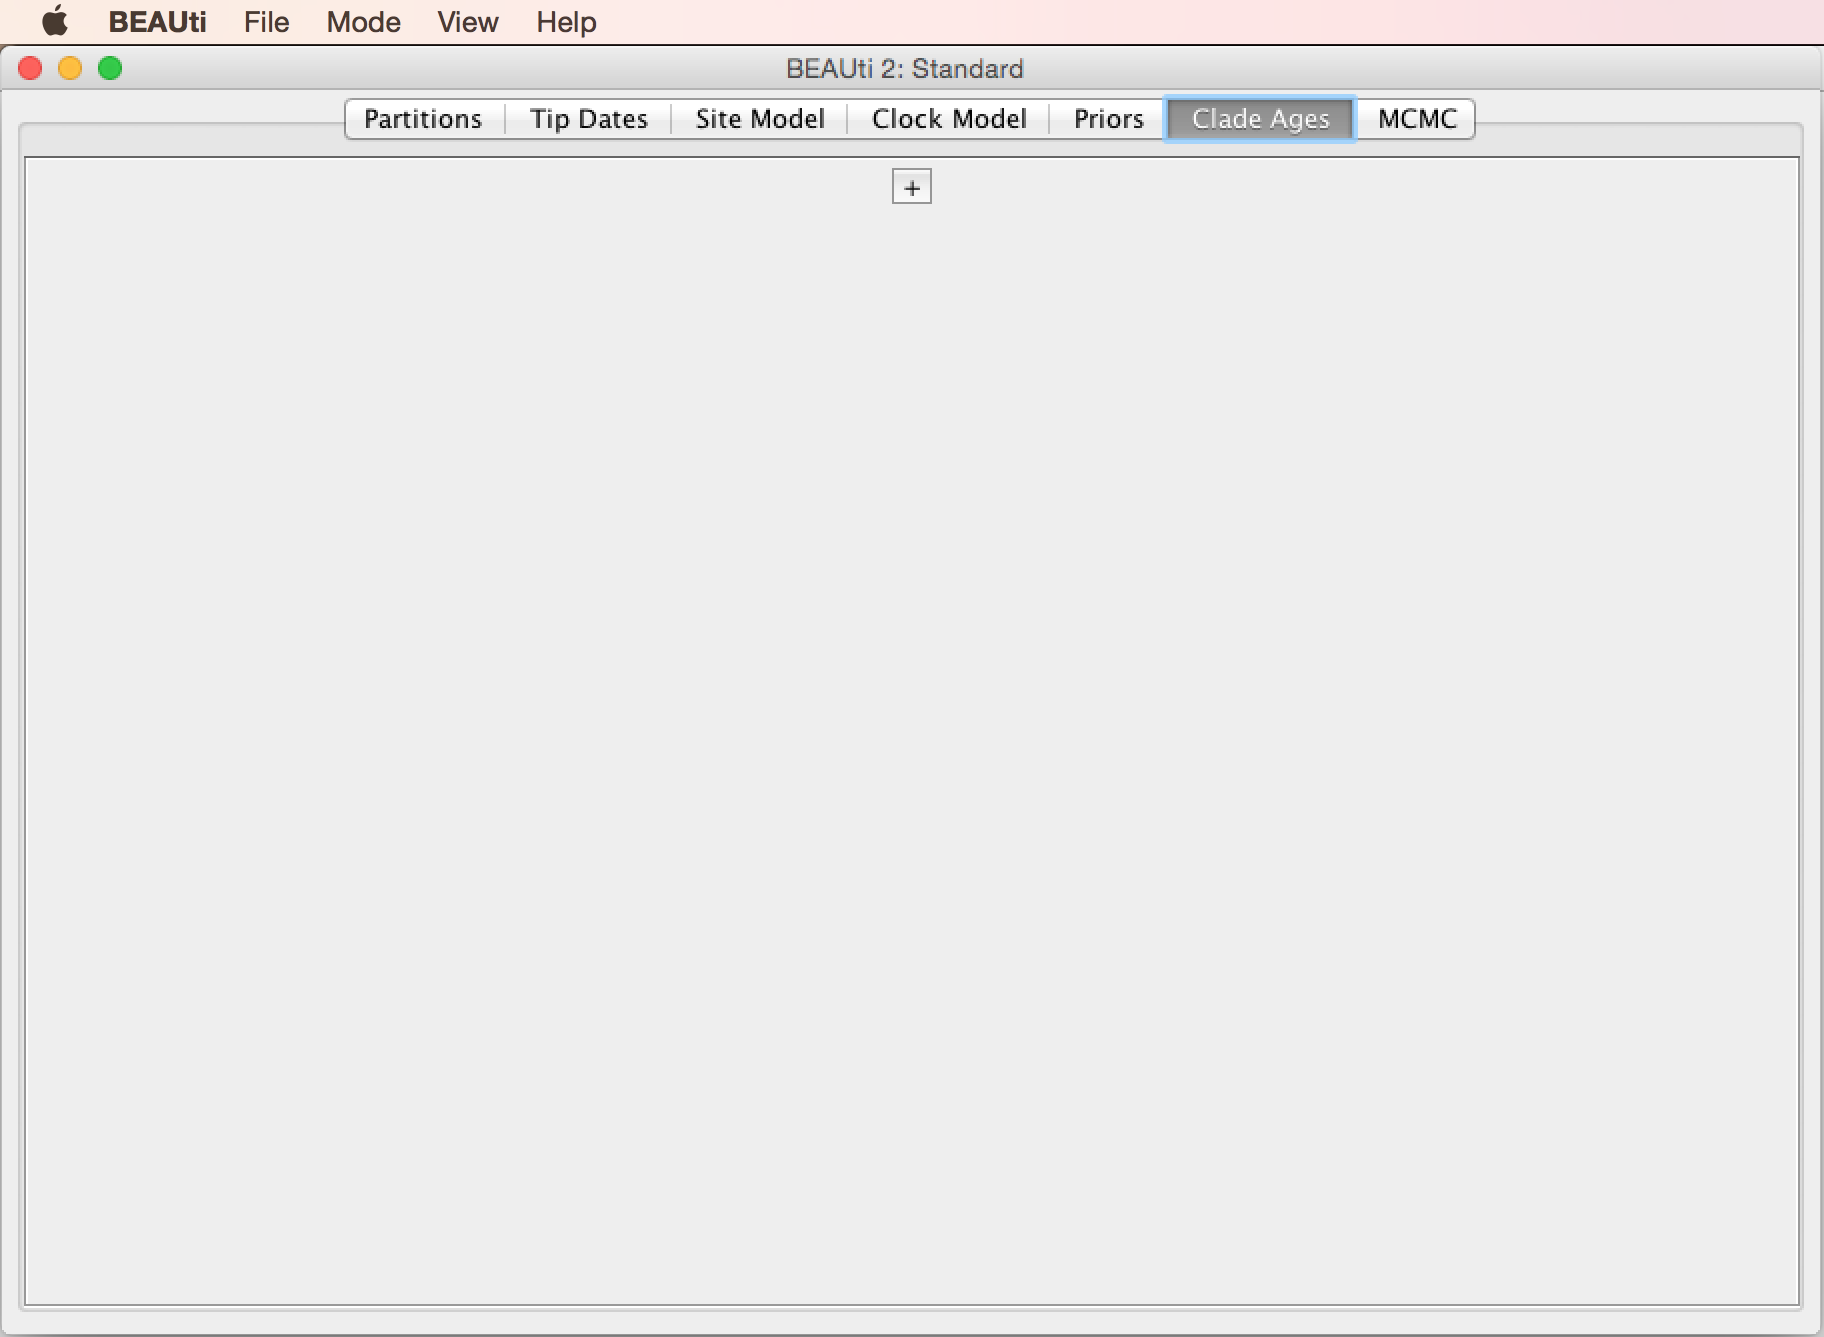
\includegraphics[width=\textwidth]{fig5.png}\end{center}

\newpage
\noindent
To specify a taxon set click on the little `+' button in the middle of the window. A new pop-up window will appear:

\begin{center}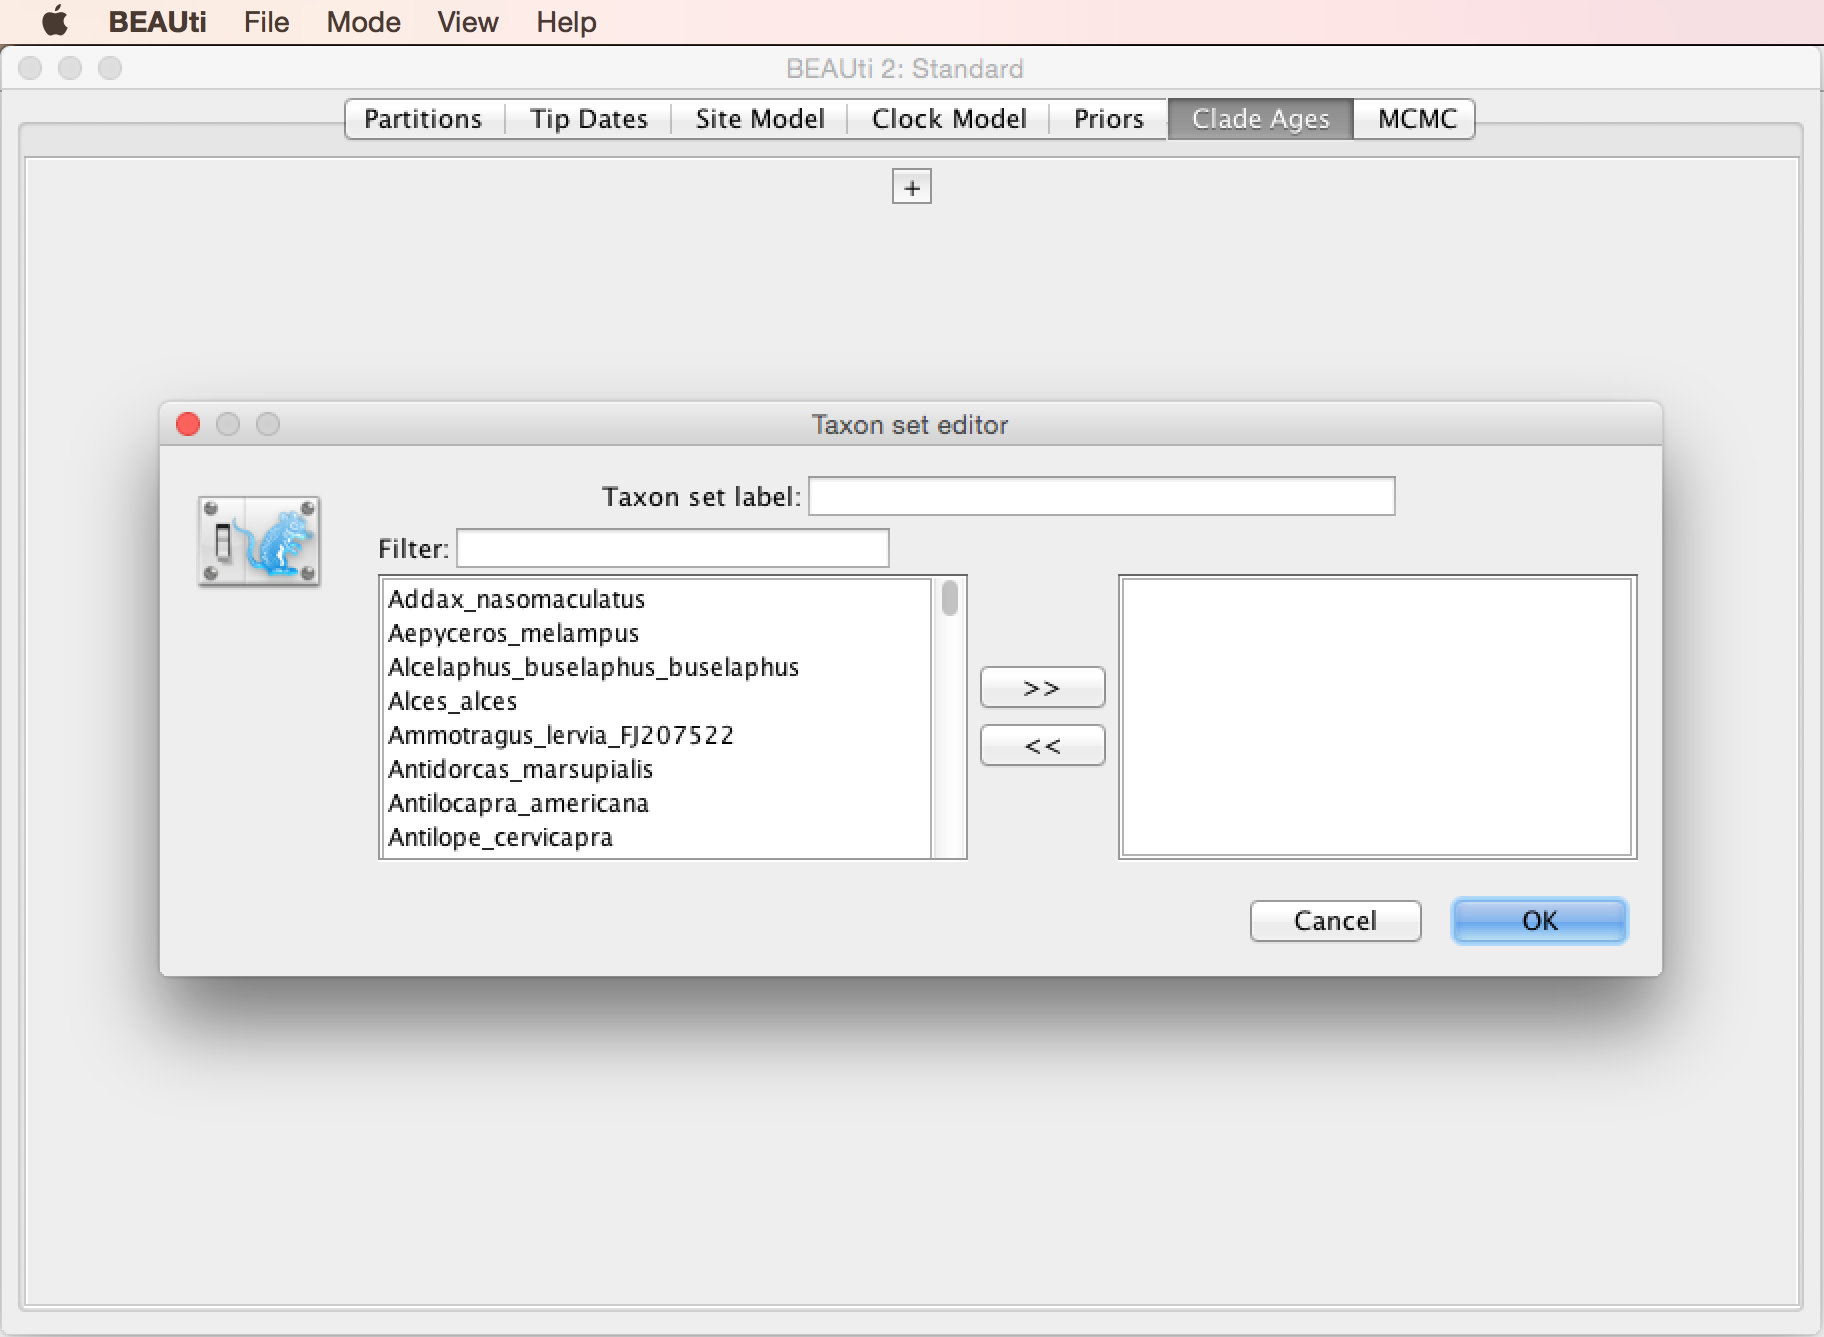
\includegraphics[width=\textwidth]{fig6.png}\end{center}

\noindent
The dataset used in this example is an alignment of mitochondrial genome sequences of 183 species of cetartiodactyls (even-toed ungulates, including ceta\-ce\-ans) \citep{Hassanin:2012il}. To constrain the age of origin of cetaceans with the fossil $\dagger$\textit{Himalayacetus subathuensis} (see \ref{first_occurrence_age}), a taxon set comprising all cetaceans first needs to be specified. To do so, provide a taxon set label (here \emph{Cetacea}), select taxa that are part of this clade, and click the `\textgreater\textgreater' button to move these into the ingroup.

\begin{center}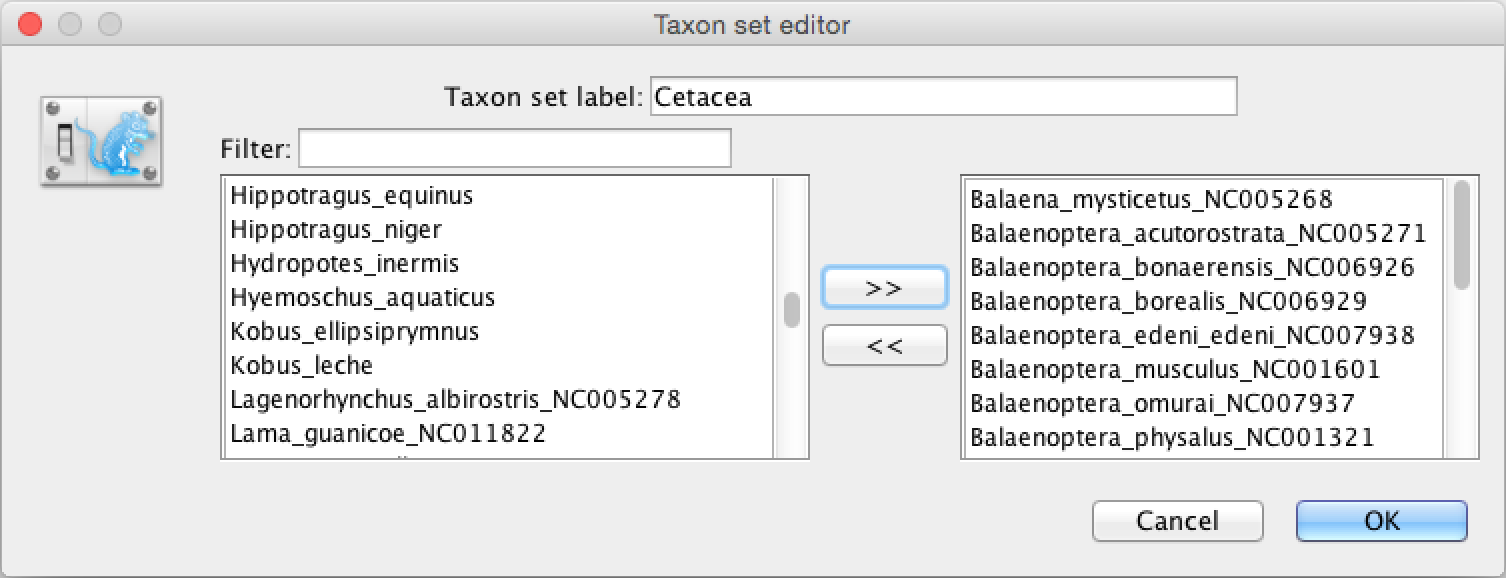
\includegraphics[width=0.825\textwidth]{fig7.png}\end{center}

\noindent
Click \emph{OK}.

\newpage
\noindent
The \emph{Clade Ages} panel should then look similar to this:

\begin{center}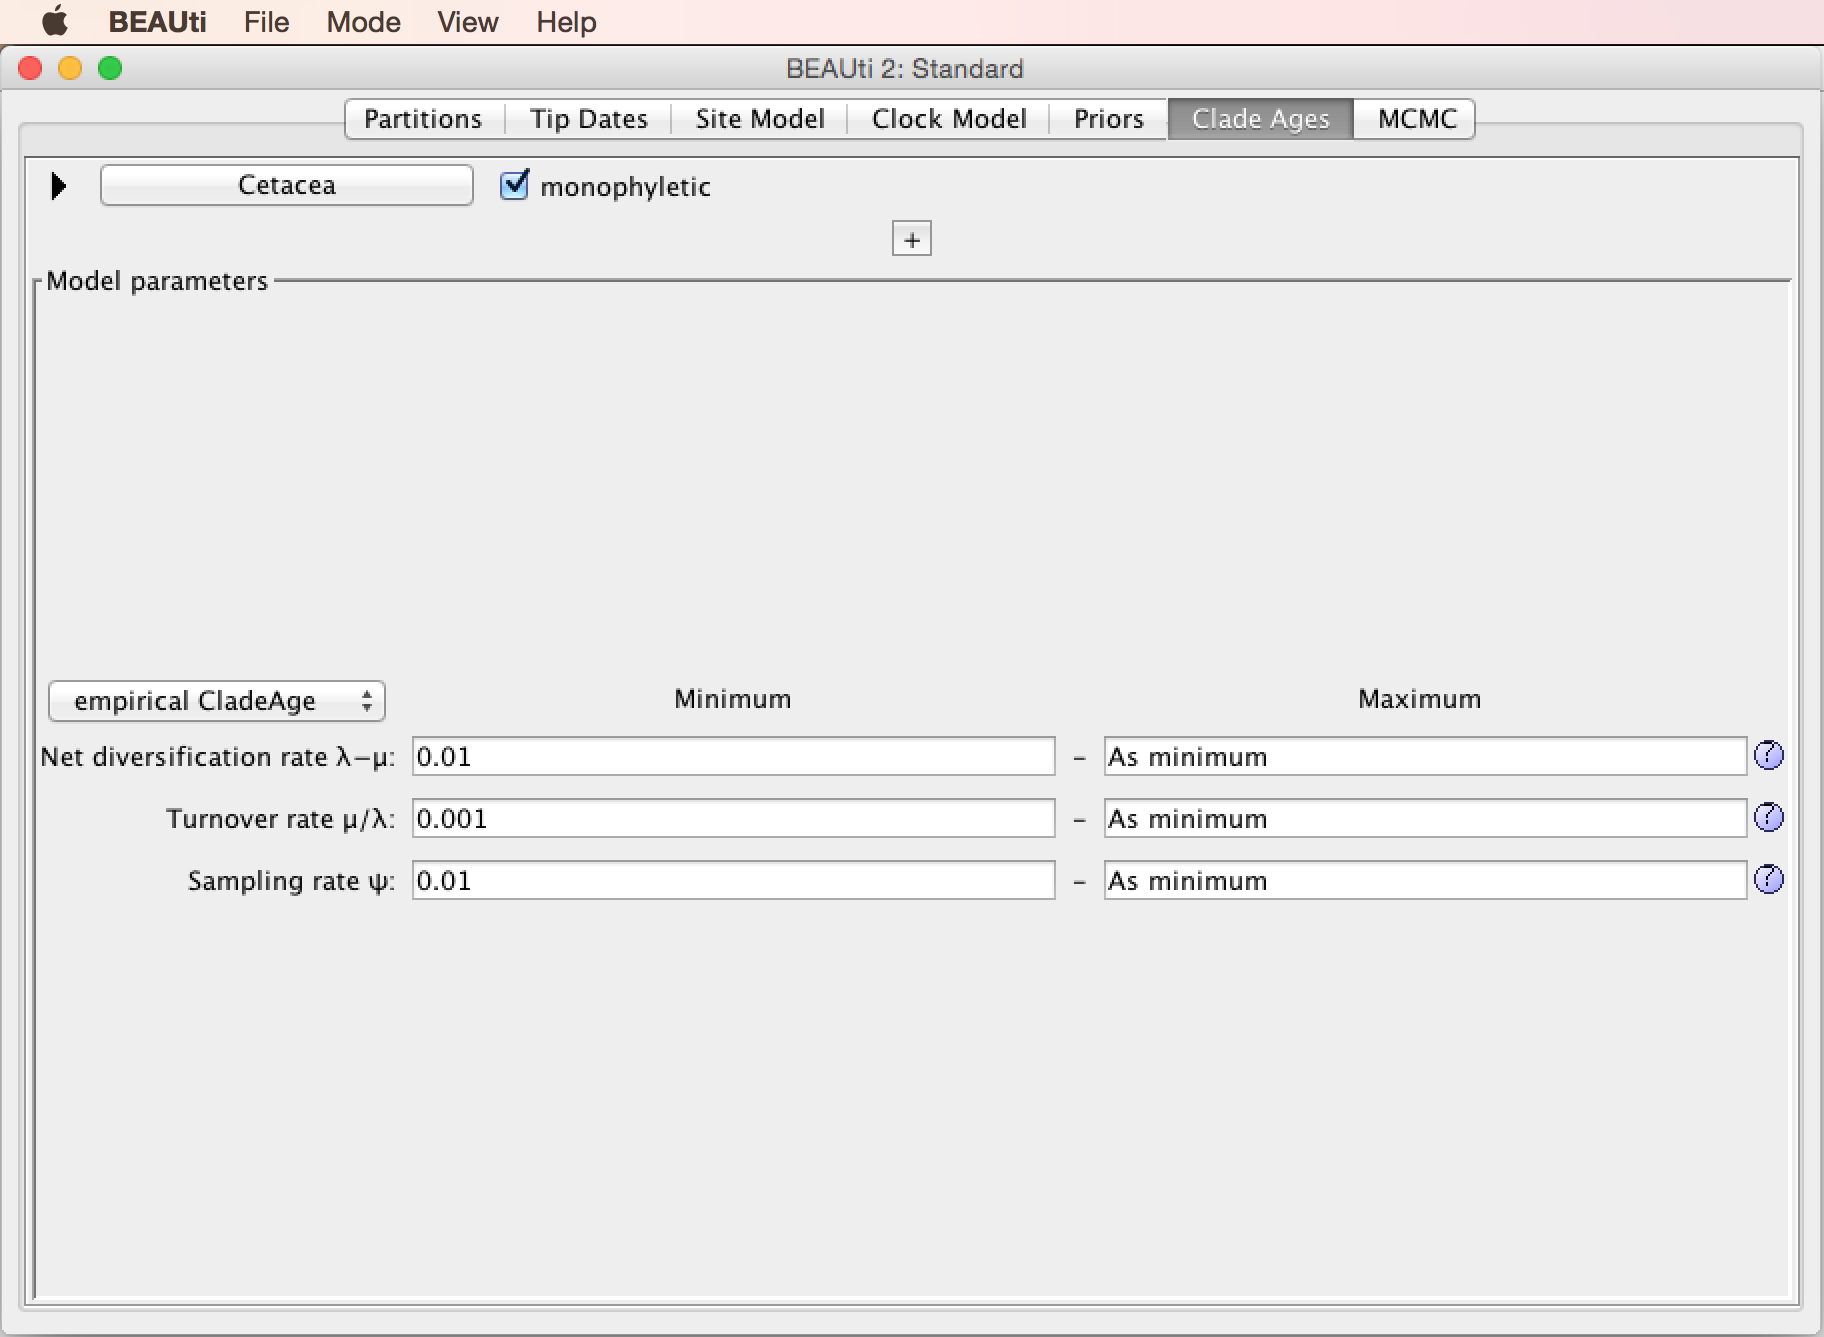
\includegraphics[width=\textwidth]{fig8.png}\end{center}

\noindent
Here, you can specify estimates for the net diversification rate, the turnover rate, and the sampling rate. If both minima and maxima are specified for these parameters, CladeAge will account for the uncertainty of in the rate estimates. If only a minimum is specified, it will be considered as a point estimate without uncertainty. The default values for these parameters should not be trusted, instead you should identify reasonable estimates for all three parameters from the literature or based on separate analyses (see \ref{diversification_rates} and  \ref{sampling_rate}).

The specified rates for net diversification, turnover, and sampling will be used for all CladeAge calibration densities specified through BEAUti, thus assuming that all clades included in the dataset share the same characteristics of diversification and preservation. This assumption may be unrealistic for large phylogenies including highly divergent groups. To specify different rates for different clades, the XML file produced by BEAUti can be edited as described in \ref{manual_spec}.

If you click on the question marks to the right of the input fields, more information will be provided in a pop-up window. The drop-down menu just above \emph{Net diversification rate} indicates the type of CladeAge calibration density. The \emph{empirical CladeAge} densities should be fine for all purposes (but if you're interested in the alternative options, please see \ref{calibration_types}).

At the top left of the panel, you'll see a field with the specified name of the clade (here \emph{Cetacea}). The checkbox to the right of this field indicates that by default clades used for fossil calibrations are expected to be monophyletic. If you uncheck this box, the topology of the taxa included in the clade will not be constrained. However, clades for which monophyly is questionable should not be constrained in the first place, as the assignment of fossils to these clades is unlikely to be reliable if the clade itself is not monophyletic. Thus, we advice to leave the \emph{monophyletic} checkbox set.

To specify the first occurrence age (and the sampling gap) for this clade, click on the little triangle to the left of the field with the clade name (\emph{Cetacea}). A new part of the panel will open:

\begin{center}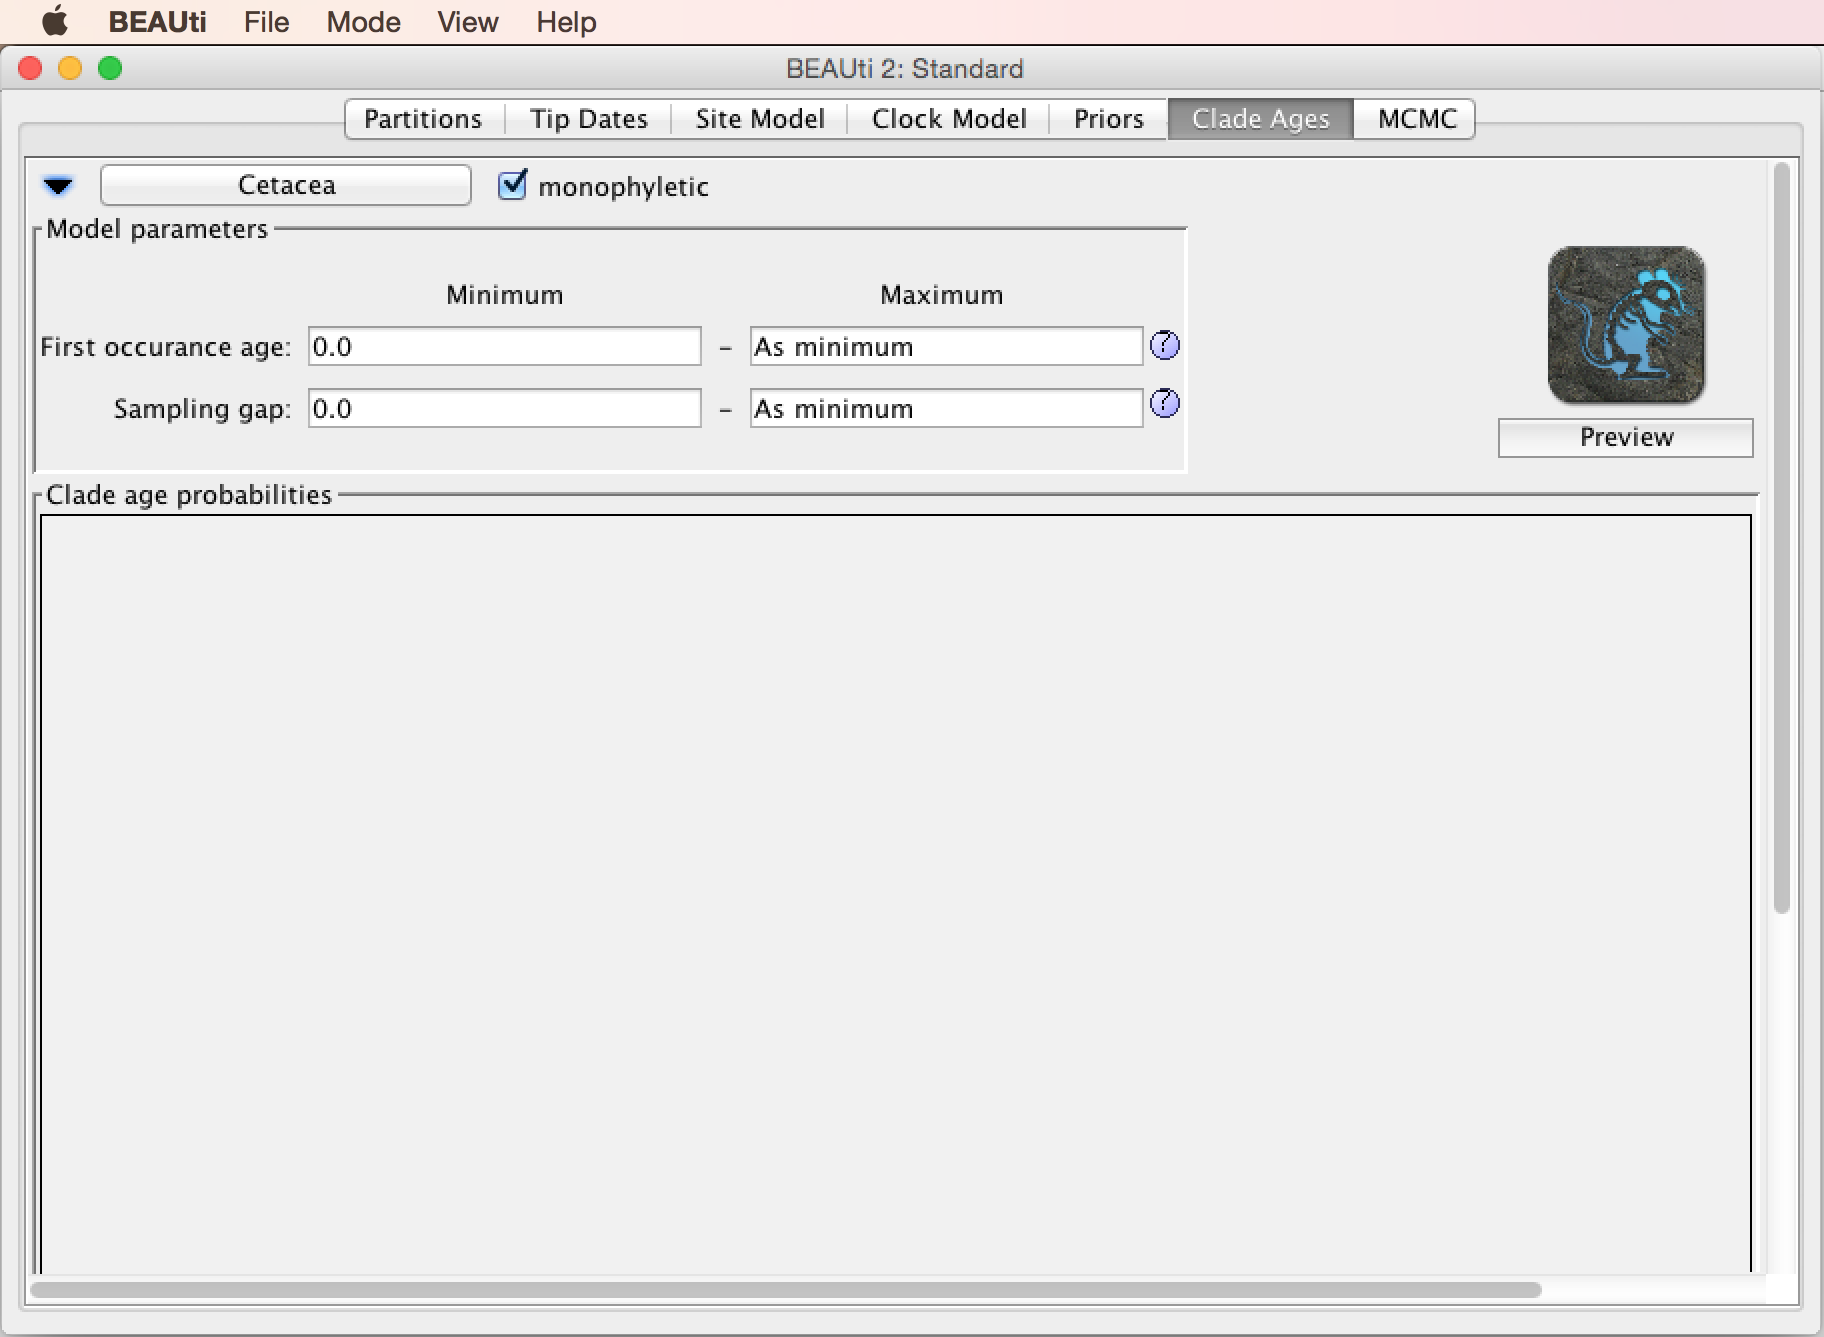
\includegraphics[width=\textwidth]{fig9.png}\end{center}

\noindent
Enter the minimum and maximum for the first occurrence age. If no maximum is provided, the minimum will be used as a point estimate, assuming that the fossil age is known exactly. To ignore the sampling gap, just leave the minimum and maximum fields as they are. Again, more information about the two parameters can be displayed by clicking on the question marks to the right of the input fields. To see the shape of the CladeAge calibration density calculated on the basis of all specified parameters, click the \emph{Preview} button below the CladeAge icon. The density shown in the figure on the next page is based on a first occurrence age between 56.0 and 53.5 million years, and more or less arbitrarily chosen point estimates for net diversification rate (0.04 per million year), turnover rate (0.5), and sampling rate (0.05 per million year).

\begin{center}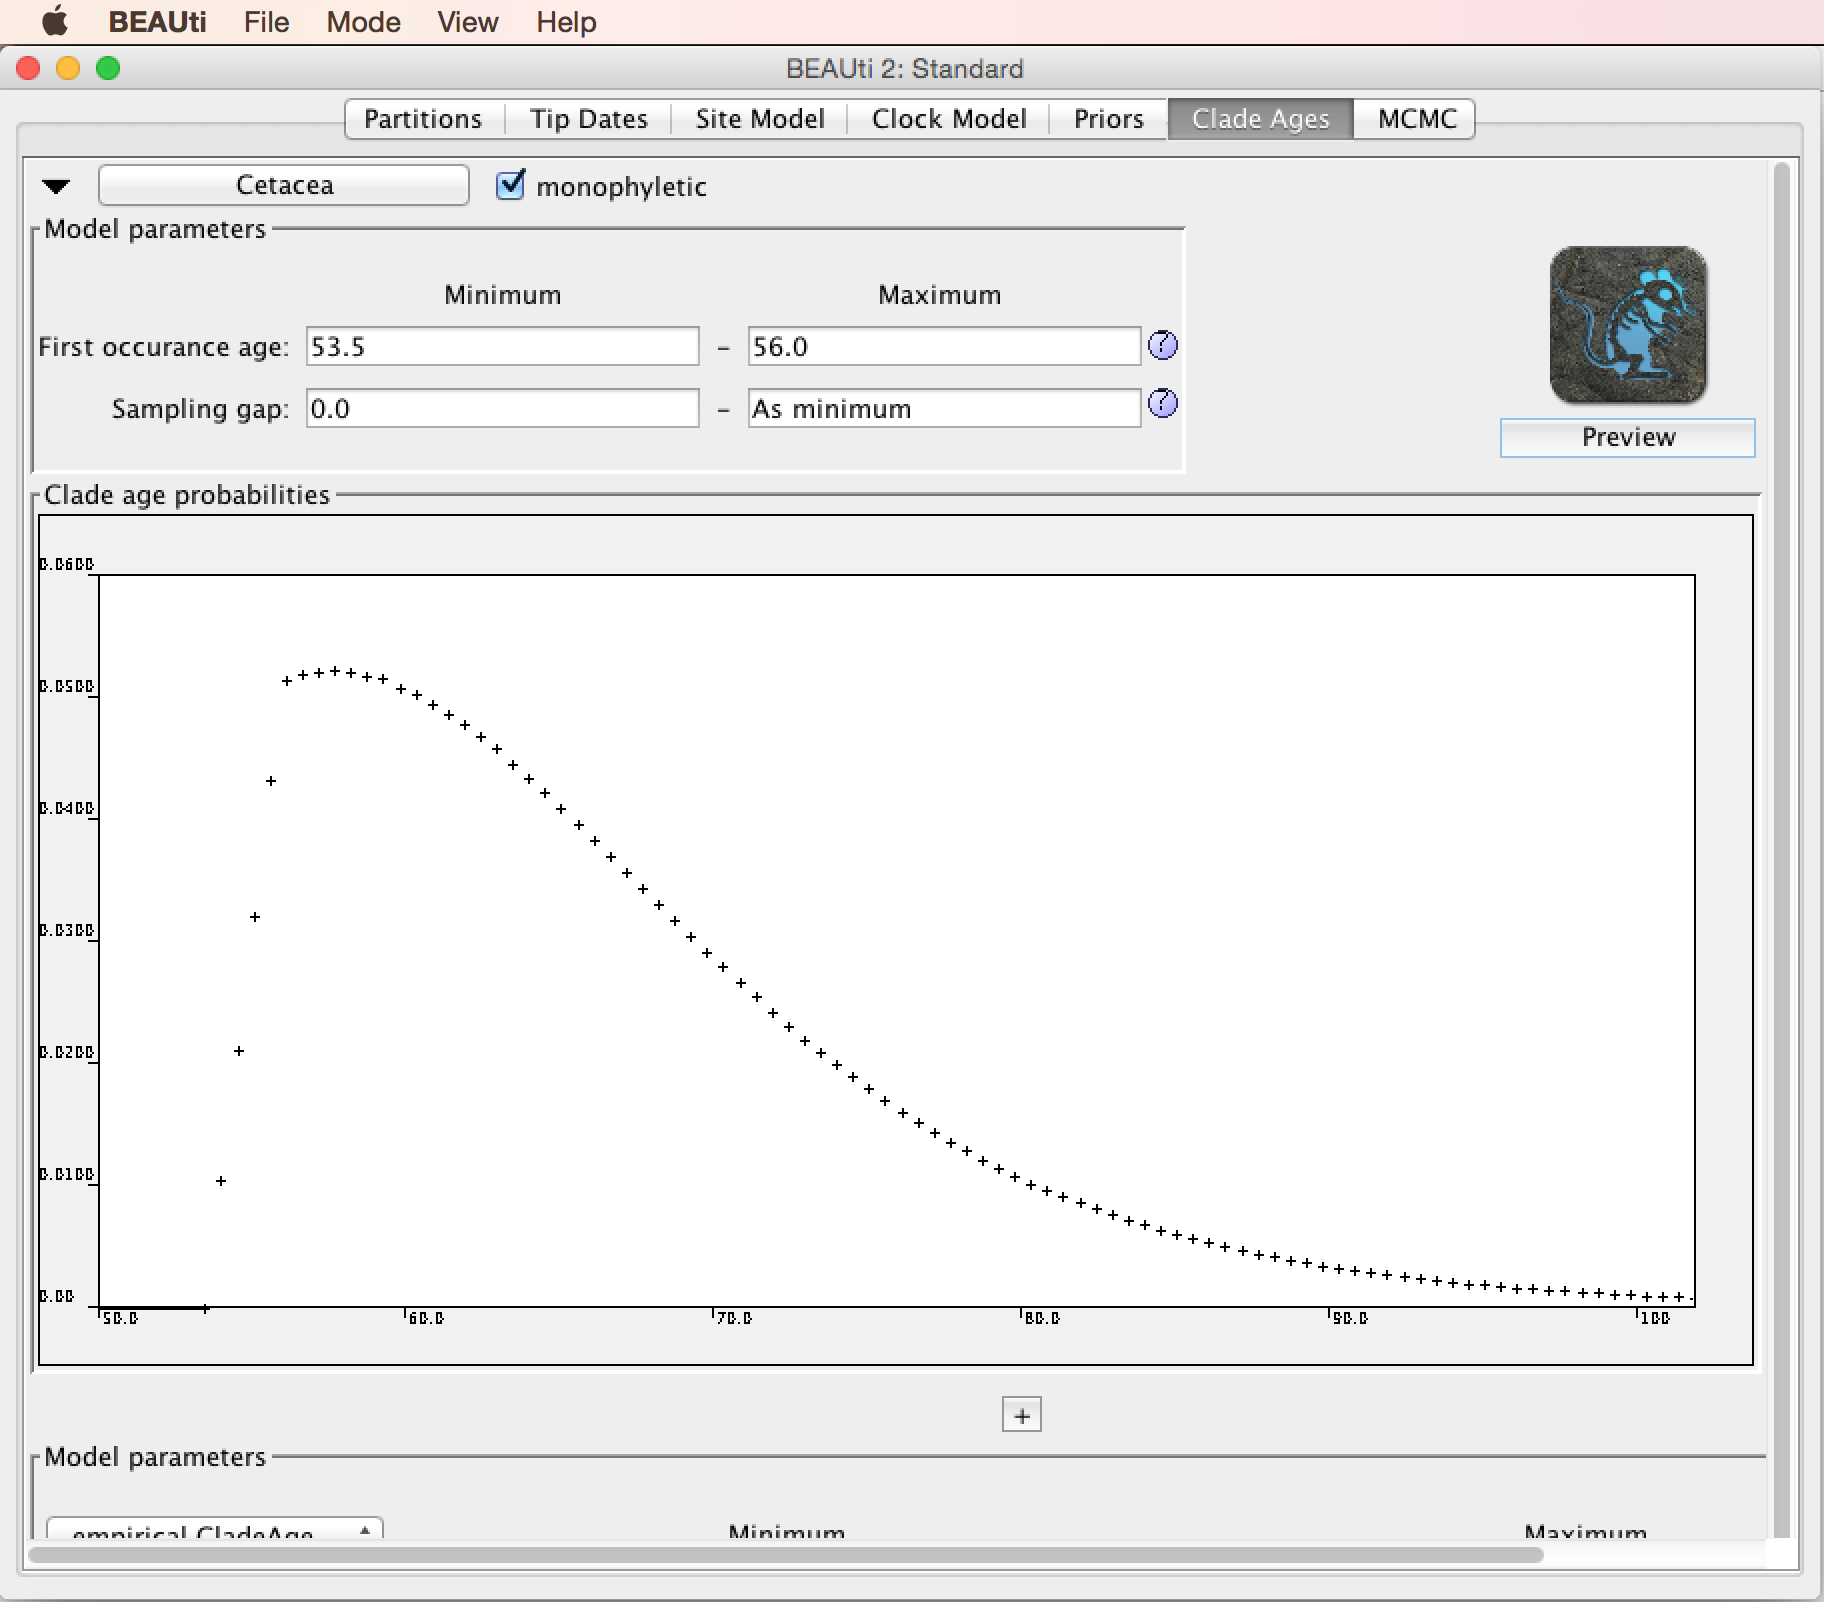
\includegraphics[width=\textwidth]{fig10.png}\end{center}

\noindent
To specify calibration densities for additional clades, click the triangle at the top left again to collapse the information for the first calibration density, and click little `+' button in the middle of the window once again. Once you have specified constraints for all clades, don't forget to set all other options for BEAST 2 analyses in the panels \emph{Site Model} and \emph{Clock Model} and check the prior distributions in the \emph{Priors} panel. Then, set the length of the MCMC in the \emph{MCMC} panel and save the XML file for BEAST 2 (more information on these settings can be found, e.g., in the \emph{Divergence Dating} tutorial available from \href{http://beast2.org/tutorials/}{http://beast2.org/tutorials/}).

\subsection{Manual specification in the XML}\label{manual_spec}

Obviously, BEAUti is just one way to produce XML input files for BEAST 2. You could also prepare XML files manually by modifying the examples provided in the \emph{examples} folder that comes as part of the BEAST 2 download, or you could use a script such as BEASTmasteR (\href{https://github.com/nmatzke/BEASTmasteR}{https://github.com/nmatzke/BEAST\- masteR}; a similar script is provided here: \href{https://github.com/mmatschiner/Introgression-Tutorial}{https://github.com/mmatschiner/\allowbreak Introgression-Tutorial}). However, if the XML is prepared in any other way than with BEAUti, CladeAge calibration densities will also have to be added to the XML code manually.

\noindent
The following code block, which is placed inside the \emph{posterior} distribution element, specifies a CladeAge calibration density in the XML file. As you can see, changing the minimum and maximum for any of the CladeAge model parameters is rather straightforward - for example, to change the minimum and maximum sampling rate, just replace \emph{0.05} after \emph{minSamplingRate} and \emph{maxSampling\-Rate} with another value.

\footnotesize
\begin{verbatim}
<distribution id="fossilCalibrations" spec="util.CompoundDistribution">
  <distribution id="Cetacea.fossilprior"
      spec="beast.math.distributions.FossilPrior"
      monophyletic="true" tree="@Tree.t:id">
    <fossilDistr id="FossilCallibration.0"
        spec="beast.math.distributions.FossilCalibration">
      <parameter id="RealParameter.0" name="minOccuranceAge">53.5</parameter>
      <parameter id="RealParameter.01" name="maxOccuranceAge">56.0</parameter>
      <parameter id="minDivRate" name="minDivRate">0.04</parameter>
      <parameter id="maxDivRate" name="maxDivRate">0.04</parameter>
      <parameter id="minTurnoverRate" name="minTurnoverRate">0.5</parameter>
      <parameter id="maxTurnoverRate" name="maxTurnoverRate">0.5</parameter>
      <parameter id="minSamplingRate" name="minSamplingRate">0.05</parameter>
      <parameter id="maxSamplingRate" name="maxSamplingRate">0.05</parameter>
      <parameter id="RealParameter.02" name="minSamplingGap">0.0</parameter>
      <parameter id="RealParameter.03" name="maxSamplingGap">0.0</parameter>
    </fossilDistr>
    <taxonset id="Cetacea" spec="TaxonSet">
      <taxon id="Balaena_mysticetus_NC005268" spec="Taxon"/>
      <taxon id="Balaenoptera_acutorostrata_NC005271" spec="Taxon"/>
      <taxon id="Balaenoptera_bonaerensis_NC006926" spec="Taxon"/>
      ... (a list of all taxon ids included in this clade) ...
      <taxon id="Tursiops_truncatus_NC012059" spec="Taxon"/>
    </taxonset>
  </distribution>
</distribution>
\end{verbatim}
\normalsize

\noindent

To specify multiple CladeAge calibration densities, one could simply copy paste the above code block several times, each time replacing the species ids in the \emph{taxonset} element, depending on which species are part of the calibrated clade. When doing so, one should also take care to change the id of the \emph{taxonset} element (which says \emph{Cetacea} in the code block example). Additionally, the id of the \emph{distribution} element that says \emph{Cetacea.fossilprior} in the example should be changed as well as the id of the \emph{fossilDistr} element (which is \emph{FossilCallibration.0} in the example code). Furthermore the ids of the \emph{parameter} elements (which are \emph{RealParameter.0}, \emph{RealParameter.01}, \emph{minDivRate}, etc.\ in the example) will need to be modified in copied blocks, and of course parameter values may need to be adjusted. It does not matter what the ids are replaced with (as they will not be referred to by other elements), they should be changed only for the reason that the same ids are not used for multiple elements (which would cause BEAST 2 to stop the run). Also note that the tree id \emph{Tree.t:id} to which the `\emph{Cetacea.fossilprior}' distribution element refers to will need to be changed to match the actual tree id specified in the XML.

\section{Types of CladeAge calibration density distributions}\label{calibration_types}

If you've been wondering what the difference is between the different types of CladeAge calibration density distributions available through BEAUti (\ref{using_beauti}), the following descriptions may be helpful. However, note that the so-called \emph{empirical CladeAge} distributions which are used by default have been thoroughly tested and there's currently no reason to use any other types of CladeAge distributions instead. So, the below descriptions are given mostly for the sake of completeness and can safely be skipped.

What all types of CladeAge calibration density distributions have in common is that they are based on calculations of the clade age probability density for 100 time points between the minimum first occurrence age of the clade and a maximal time point that is predetermined based on a quick approximation \citep[details given in][]{Matschiner:2016ga}. However, the difference between the types of CladeAge distributions lies in the way in which these 100 calculated densities are turned into probability density distributions.

\begin{itemize}
\item
{\bf Empirical CladeAge distributions}: In the default \emph{empirical CladeAge distributions}, the calculated probability densities are used directly for the respective time points. Probability densities for times in between these time points are interpolated from the probability densities of the two neighbouring time points, using a linear regression. For all times older than the oldest sampled time point (the tail of the distribution), probability densities are approximated by an exponential distribution that is calculated on the basis of the two oldest time points, so that the probability densities calculated for these two time points lie on this exponential distribution. Finally, \emph{empirical CladeAge distributions} are scaled so that the total probability mass becomes 1. \emph{Empirical CladeAge distributions} are the only available distribution type when a sampling gap (see \ref{sampling_gap}) is specified.

\item
{\bf Fitted CladeAge distribution}: CladeAge allows the fitting of what we call \emph{fitted CladeAge distributions} to the calculated probability densities. These distributions are similar to truncated lognormal distributions, except that the parameterisation is simplified. The probability density function of an \emph{fitted CladeAge distribution} is as follows:

\begin{equation*}
f_{u} =
\begin{cases}
0, & \mbox{if } u \leq 0 \\
\frac{c}{u + s} \times e^{\frac{-(\mathrm{ln}(u+s) - m)^2}{w}}, & \mbox{if } u > 0,
\end{cases}
\end{equation*}

where $u = t_o - t_f$ and parameters $c$, $s$, $m$, and $w$ (all $\geq 0$) can be optimised so that $f_{u}$ fits the calculated probability densities and its integral sums to 1. We have chosen to introduce this type of distribution, because we found truncated lognormal distributions to provide a near-perfect fit to the calculated probability densities, however the parameterisation of lognormal distributions makes analytical handling unnecessarily complicated. While providing the same fit as truncated lognormal distributions, the simplified parameterisation of \emph{fitted CladeAge distributions} facilitates analytical solution of distribution parameters, as well as analytical integration of the distribution.

Knowing the integral of a distribution is necessary in order to analytically account for uncertainty in the age of first occurrence. The integral of an \emph{fitted CladeAge distribution} is

\begin{equation*}
\int_0^a \! f_{u} \, \mathrm du=
\begin{cases}
0, & \mbox{if } a \leq 0 \\
-\frac{c \sqrt{\pi w}}{2} \times \erf(\frac{m - \mathrm{ln}(a+s)}{w}), & \mbox{if } a > 0,
\end{cases}
\end{equation*}

where erf is the error function, which CladeAge calculates via a numerical approximation with a maximal error of $1.2 \times 10^{-7}$ \citep{Press:2007vx}.

The analytical solution of the parameters of an \emph{fitted CladeAge distribution} is possible when probability densities of only 4 instead of 100 time points are considered, and the fit of the distribution is only slightly worse if these four time points are carefully selected \emph{a priori}. This massively reduces computation time not only by the limited number of time points for which probability densities must be calculated, but also because the analytical solution of distribution parameters is much faster than the distribution fitting through minimisation of root mean square deviations. As a result, the time needed for the calculation of \emph{fitted CladeAge distribution} parameters is on the order of 0.005 seconds. Of course, if prior distributions are calculated just once before a time-calibration analysis, it hardly matters whether this calculation takes 0.005 s or 1 s. However, the fast analytical calculation of distribution parameters in would allow repeatedly recalculating these parameters during a BEAST run without substantial delay. In this case, diversification rates $\lambda$ and $\mu$ would not need to be specified by the user. As the BEAST MCMC estimates these parameters anyway, these estimates could be used directly for \emph{fitted CladeAge distributions}. Whenever the BEAST estimates for $\lambda$ and $\mu$ change during the MCMC run, \emph{fitted CladeAge distributions} are recalculated with the updated estimates. This feature is experimental and run-time recalculation of \emph{fitted CladeAge} distributions has not been made available yet.

\item
{\bf Standard distributions}: 
Besides \emph{empirical} and \emph{fitted CladeAge distributions}, CladeAge allows the fitting of commonly used distribution types against the calculated probability densities. Available distributions include {\bf exponential}, {\bf lognormal}, {\bf normal} and {\bf gamma distributions}. These distributions are scaled during the fitting process, however the scaling factor is not reported and should be ignored when these distributions are used as priors in Bayesian analyses, otherwise the probability mass of the distribution would not sum to 1.

\if0 TRUNCATED DISTRIBUTIONS ARE NOW DEPRECATED
\item
{\bf Truncated standard distributions}: If the first occurrence age is known without uncertainties (see section 2.5), {\bf truncated lognormal}, {\bf truncated gamma}, and {\bf truncated normal distributions} can be fitted to the calculated probability densities. As with untruncated distributions, these are scaled during the fitting process and the scaling factor is not reported, but unlike untruncated distributions, truncated distributions will not sum to 1 anyway. {\bf This is work in progress, and this option is not yet available in BEAST}.
\fi
\end{itemize}

% The following command tells Bibtex to use the bibliography style sheet designed specifically for Molecular Ecology.
% This style sheet must be either in the directory of the manuscript, or in a bst folder that is something like
% /usr/local/texlive/2007/texmf-dist/bibtex/bst
\bibliographystyle{molecol}

% The following command includes references listed in the file references.bib, which should be in the same folder as the manuscript.
\bibliography{references}

\end{document}
